\section{Introduction}
\emph{We are given an array that contains N numbers and would like to determine if there are two numbers whose sum equals a given number K.\\
For example we may be given the sequence 4,1,5,2,6,3 and are asked to find a pair of numbers with a sum of 10. In this example 4 and 6 is a valid result.\\
To solve the portfolio do the following:}
\begin{itemize}

\item \emph{Implement an O\(\left( { N }^{ 2 } \right)\) algorithm for solving the problem.}
\item \emph{Implement an O\(\left( N\log {(N)}  \right) \) algorithm for solving the problem. (Hint: Consider sorting the list.)}
\item \emph{Perform experiments with different values of N (generate the associated random lists yourselves)
and plot the time as function of N, to verify the time complexity.}
\end{itemize}
\emph{You may use a build in sorting algorithm and assume that it sorts in \( N\log {(N) }  \).}

\section{Use of Algorithms}
A description of the algorithms mentioned in Section \ref{sec:algorithm1} and \ref{sec:algorithm2}. 
The complexity of the algorithms is verified in Section \ref{sec:ver}.
The source code of the algorithms used to solve the problem is showed in Appendix \ref{app:matcher}.


\subsection{O\(\left( { N }^{ 2 } \right)\) Algorithm}
\label{sec:algorithm1} 
\todo[inline]{Description af the algorithm}
\todo[inline]{Pseudocode}


O\(\left( { N }^{ 2 } \right)\)

O\(\left( N\log {(N)}  \right) \)

\( \log {(N)} \)


\subsection{O\(\left( N\log {(N)}  \right) \) Algorithm}
\label{sec:algorithm2}
The problem is solved using a binary search algorithm. A requirement for the binary searching algorithm is that the vector of number has to be sorted, before a binary search algorithm can be applied. \\
The algorithm starts by checking the first value of the vector, and calculates, what value it needs to pair up with to get a sum of \emph{K}.  Using binary search the needed value will be found in the vector, if the value isn't found in the vector, the next value will be checked.  When a pair is found the algorithm \emph{return 1}. \\

The binary search algorithm in use is a build in algorithm which is available from the standard library \emph{algorithm.h}. The binary search algorithm is a bool, which return true or false depending whether or not it finds the value. The algorithm itself takes 3 parameter, a iterator pointing to first element, a iterator pointing to last element, and the value which has to be found. 
\begin{lstlisting}
binary_search(v.begin(), v.end(), find_value)
\end{lstlisting}

\newpage
\section{Verify the Time Complexity for the Algorithms}
\label{sec:ver}
One hundred lists with elements in range of [1000 100000] are used for testing the worst case complexity of the algorithms. To get the worst time case the "search number" must not be included as a element, therefore the lists are not random generated. 

\subsection{O\(\left( { N }^{ 2 } \right)\) Implementation}
Figure \ref{fig:test1} shows an ideal O\(\left( { N }^{ 2 } \right)\) complexity and the data samples is plotted, time as function of elements. If you compare the plots according to the rate of change the curves are exactly alike. \\

\begin{figure}[th!]
\centering
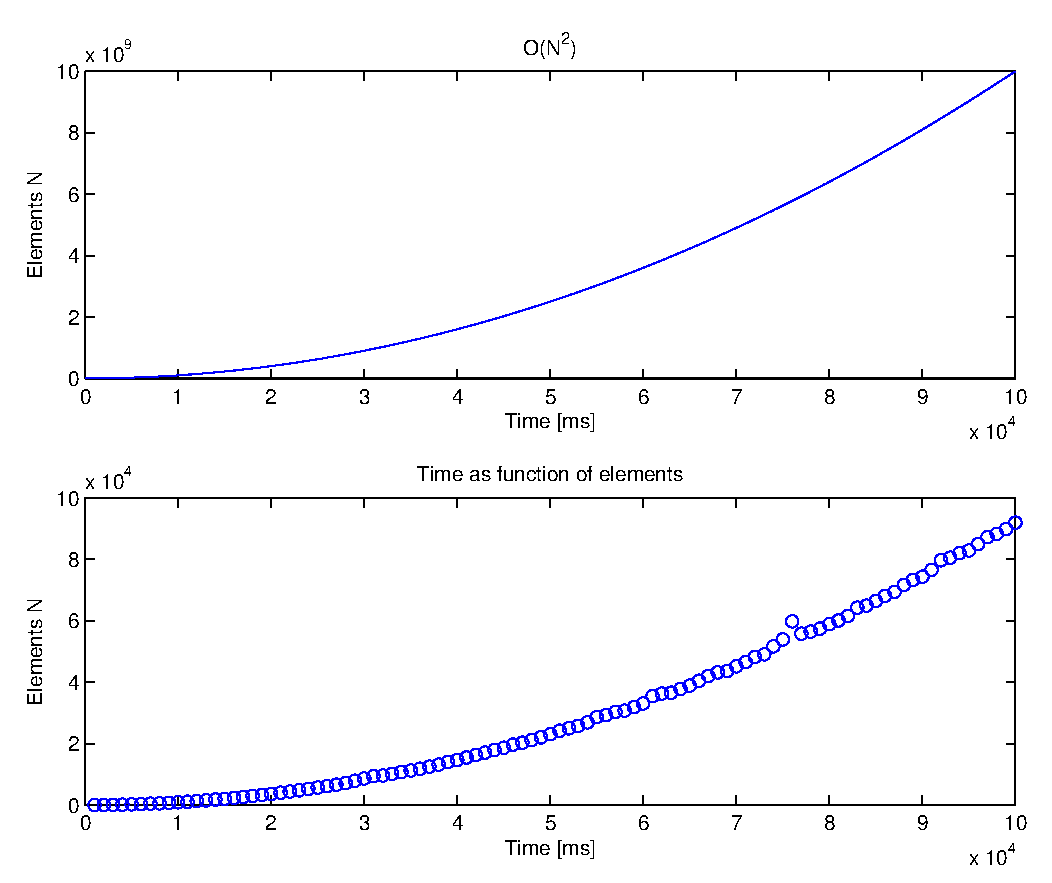
\includegraphics[width=1\textwidth]{./graphics/test1.eps}
\caption{Show plots of an ideal O\(\left( { N }^{ 2 } \right)\) complexity and data samples from the used algorithm.}
\label{fig:test1}
\end{figure}

The complexity in worst case is: O\(\left( { N }^{ 2 } \right)\), since array has to be looked through twice for a match. 


\newpage
\subsection{O\(\left( N\log {N }  \right) \) Implementation}
Figure \ref{fig:test2} shows an ideal O\(\left( N\log {N }  \right) \) complexity and the data samples plotted as time as function of elements. If you compare the plots according to the rate of change the curves they are exactly alike. 
\begin{figure}[th!]
\centering
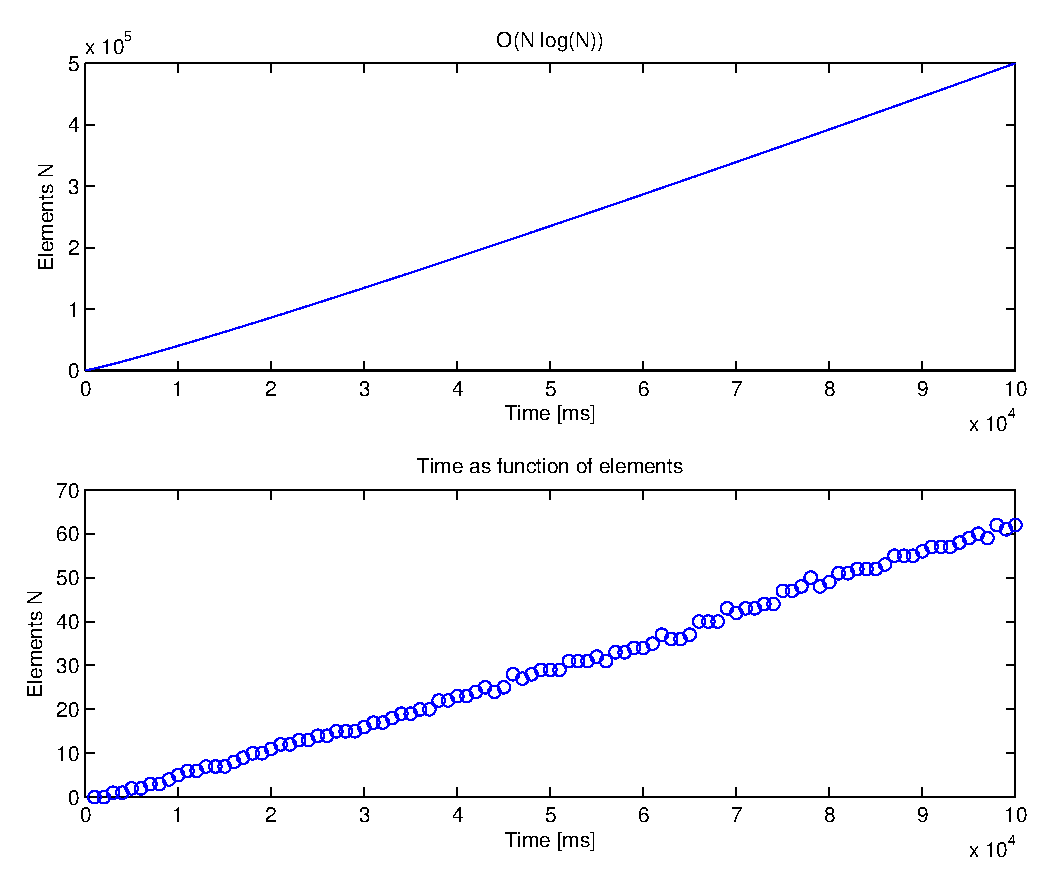
\includegraphics[width=1\textwidth]{./graphics/test2.eps}
\caption{Show plots of an ideal O\(\left( N\log {N }  \right) \) complexity and data samples from the used algorithm.}
\label{fig:test2}
\end{figure}

The complexity is in worst case O\(\left( N\log {(N)}  \right) \), since the worst case implies that the whole array has to be looked through. And using binary search the searching itself has the complexity \( \log {(N)} \). Thereby the algorithm is fulfilling the criteria of having a complexity of O\(\left( N\log {(N)}  \right) \).  


\section{Conclusion}
By using two different algorithms to find matching numbers in the same data structures it is necessary to think about the complexity of the algorithm. As illustrated in Figure \ref{fig:test1} and Figure \ref{fig:test1}, a implementation with the worst case complexity O\(\left( N\log {(N)}  \right) \) is appropriate for this giving problem.
